\documentclass[spanish, a4paper, 12pt, openany,final]{book} 
\usepackage{textcomp}
\usepackage[T1]{fontenc, url}
\usepackage[utf8]{inputenc}
\usepackage{titlesec}
\setcounter{secnumdepth}{4}
\usepackage{multirow}      
\usepackage{algpseudocode} 
\usepackage{datetime2}
\usepackage{multicol}
\usepackage[Algoritmo]{algorithm}               
\usepackage{minted}                             
\usepackage{adjustbox}                          
\usepackage{graphicx}                           
\usepackage{amsmath, amssymb, amsthm}           
\usepackage{parskip}                            
\urlstyle{sf}                                   
\usepackage{color}                              
\usepackage{subcaption}                         
\usepackage[toc,page]{appendix}                 
\usepackage{chngcntr}                   
\usepackage{verbatim}        
\counterwithout{figure}{section}
\counterwithout{figure}{chapter}        
\counterwithout{table}{section}
\counterwithout{table}{chapter}    
\counterwithout{equation}{chapter}    
\counterwithout{equation}{section}
\hyphenpenalty=100000                           
\sloppy                                         
\raggedbottom                                   
\usepackage{xparse,nameref}                     
\usepackage[bottom,hang,flushmargin]{footmisc}  
\interfootnotelinepenalty=10000                 
\usepackage{lipsum}                     

% --------- Editar de aquí en adelante --------

% ----- Apariencia e idioma ----- 
\usepackage[spanish,mexico]{babel}
\graphicspath{{Images/}{../Images/}}                                % Dónde estarán las imágenes
\usepackage[left=2.5cm,top=4cm,bottom=2.5cm,right=2.5cm]{geometry}    % Márgenes del documento
\usepackage{setspace}                                               % Permite elegir el interlineado
\linespread{1.3}                                                    % Interlineado de uno y medio. 1.6 es interlineado doble.
\usepackage{microtype}       
\usepackage{chngcntr}
   

\renewcommand{\thefigure}{\arabic{figure}}
\addto\captionsspanish{\renewcommand{\listtablename}{Índice de Tablas}}
\addto\captionsspanish{\renewcommand{\listfigurename}{Índice de Figuras}}
                        % Permite la modificación de los caracteres.


% ----- Secciones ----- % ESTA PARTE SE UTILIZA EN CASO DE USAR LA CLASE ARTICLE

% \titleformat*{\section}{\LARGE\bfseries}                  % Forma del título de \section 
% \titleformat*{\subsection}{\Large\bfseries}               % Forma del  título de \subsection
% \titleformat*{\subsubsection}{\large\bfseries}            % Forma del  título de \subsubsection 

% Las siguientes tres líneas crean el comando \paragraph con la forma del título correcta.

% \titleformat{\paragraph} 
% {\normalfont\normalsize\bfseries}{\theparagraph}{1em}{}
% \titlespacing*{\paragraph}
% {0pt}{3.25ex plus 1ex minus .2ex}{1.5ex plus .2ex}
%-----------------------------------------------

% ----- Figuras y tablas ----- 
\usepackage{fancyhdr}                           % Permite formatear las cabeceras, pies, enumeración, etc.
\usepackage{subfiles}                           % Para agregar los capítulos que se escriben aparte.
\usepackage{array}                              % Para ordenar texto y ecuaciones.
\usepackage[rightcaption]{sidecap}              % Permite agregar texto lateral
\usepackage{wrapfig}                            % Permite poner figuras con texto al rededor.
\usepackage{float}                              % Permite poner figuras en cualquier lugar.
\usepackage[labelfont=bf]{caption}              % Texto en negrita para descripciones (\caption)
\usepackage{amsmath}
\usepackage{amssymb}
\usepackage[para]{threeparttable}               % Tablas vistosas, mirar antes de utilizar.
\usepackage{url}                                % Permite el uso de enlaces URL.
\usepackage[table,xcdraw,dvipsnames]{xcolor}    % Agranda la cantidad de colores.
\usepackage{makecell}                           % Ayuda en la creación de tablas
\usepackage{hhline}                             % Agranda las opciones de las líneas
\usepackage{textcomp}                           % Símbolo de derechos de autor


% ----- Referencias -----
\usepackage{natbib}                                                     % Ambiente de referencias utilizado.
\bibliographystyle{apalike}                                                 % Estilo de referencias APA.


% ----- Cabecera y pies -----
\pagestyle{fancy}                           % Se define el estilo fancy
\fancyhead[RO,LE]{\thepage}                 % Número de página en la izquierda para par y derecha para impar
\fancyhead[RE,LO]{\nouppercase{\rightmark}} % Nombre del capítulo en la derecha para par y la izquierda para impar en la cabecera
%\renewcommand{\headrulewidth}{0pt}         % Cambiar para línea más gruesa
\fancyfoot{}                                % Saca el número de la página abajo.

\fancypagestyle{plain}{                     % Se redefine el estilo automático (plain) para que calce con el resto. En particular la 1ra página de cada capítulo
\fancyhf{}                                  % Elimina la cabecera y los pies
\fancyhead[RO,LE]{\thepage}                 % Número de página en la izquierda para par y derecha para impar
\fancyhead[RE,LO]{\nouppercase{\leftmark}}  % Nombre del capítulo en la derecha para par y la izquierda para impar en la cabecera
%\renewcommand{\headrulewidth}{0pt}         % Cambiar para línea más gruesa
\fancyfoot{}                                % Elimina el número de la página abajo
}

%------------------- Cabecera del Resumen y Agradecimientos--------------

\fancypagestyle{resumen}{                   % Se redefine el estilo resumen para que calce con el resto. 
\fancyhf{}                                  % Elimina la cabecera y los pies
\fancyhead[RO,LE]{\thepage}                 % Número de página en la izquierda para par y derecha para impar
\fancyhead[RE,LO]{\nouppercase{Resumen}}    % Nombre del capítulo en la derecha para par y la izquierda para impar en la cabecera
%\renewcommand{\headrulewidth}{0pt}         % Cambiar para línea más gruesa
\fancyfoot{}                                % Elimina el número de la página abajo
}

\fancypagestyle{abstract}{                  % Se redefine el estilo resumen para que calce con el resto. 
\fancyhf{}                                  % Elimina la cabecera y los pies
\fancyhead[RO,LE]{\thepage}                 % Número de página en la izquierda para par y derecha para impar
\fancyhead[RE,LO]{\nouppercase{Abstract}}   % Nombre del capítulo en la derecha para par y la izquierda para impar en la cabecera
%\renewcommand{\headrulewidth}{0pt}         % Cambiar para línea más gruesa
\fancyfoot{}                                % Elimina el número de la página abajo
}

\fancypagestyle{agradecimientos}{                   % Se redefine el estilo resumen para que calce con el resto. 
\fancyhf{}                                          % Elimina la cabecera y los pies
\fancyhead[RO,LE]{\thepage}                         % Número de página en la izquierda para par y derecha para impar
\fancyhead[RE,LO]{\nouppercase{Agradecimientos}}    % Nombre del capítulo en la derecha para par y la izquierda para impar en la cabecera
%\renewcommand{\headrulewidth}{0pt}                 % Cambiar para línea más gruesa
\fancyfoot{}                                        % Elimina el número de la página abajo
}

% ----- Cabecera de la portada ----- 
\fancypagestyle{frontpage}{             % Se define el estilo frontpage.
	\fancyhf{}                          % Elimina la cabecera y los pies
	\renewcommand{\headrulewidth}{0pt}  % Elimina líneas en cabecera
	\renewcommand{\footrulewidth}{0pt}  % Elimina líneas en pies
	\vspace*{1\baselineskip}
	
 \fancyhead[L]{ 
\includegraphics[width=0.7in]{escudo_udec.png}\hspace{2cm}}
	\fancyhead[C]{UNIVERSIDAD DE CONCEPCIÓN
	\linebreak FACULTAD DE INGENIERÍA
    \linebreak DEPARTAMENTO DE INGENIERÍA CIVIL INDUSTRIAL}
    \fancyhead[R]{\hspace{1cm}
\includegraphics[width=0.7in]{Images/FI_Udec.png}}
	
}

% ----- Enlaces clickeables --------
\usepackage{hyperref}   % Permite que todo el documento sea clickeable.
\newcommand\myshade{85} % Permite la redefinición de colores a gusto del usuario

% Para elegir colores propios mirar los nombres relacionados con dvipsnames, aquí un url con los nombres de dvipsnames: https://www.overleaf.com/learn/latex/Using_colours_in_LaTeX

\colorlet{mylinkcolor}{DarkOrchid}   %Hiperlinks internos
\colorlet{mycitecolor}{YellowOrange} %Citas
\colorlet{myurlcolor}{Aquamarine}    %Urls

% Para dejar el documento sin texto en colores cambiar las tres líneas anteriores a Black.

\hypersetup{  %Define la forma en que se verán las cosas clickeables.
  	linkcolor  = mylinkcolor!\myshade!black,    % Aplica el color definido arriba. En este caso DarkOrchid
  	citecolor  = mycitecolor!\myshade!black,    % Aplica el color definido arriba. En este caso YellowOrange
  	urlcolor   = myurlcolor!\myshade!black,     % Aplica el color definido arriba. En este caso Aquamarine
  	colorlinks = true,                          % Elimina las cajas al rededor de lo clickeable y lo reemplaza por palabras a color.
}


%--------------------------------------------------------------------------------------------------------------------------
% ------------------------------------------ Aquí empieza el documento ----------------------------------------------------
%--------------------------------------------------------------------------------------------------------------------------
\renewcommand{\max}{\operatorname{Maximizar}}

\usepackage{tikz}
\begin{document}
\def\biblio{}   % Resetea el comando biblio, de lo contrario una lista de referencias será producida después de cada capítulo
                % resets the biblio command, if not here a new reference list will be produced after every chapter

\begin{titlepage}
	
	\newgeometry{top=1 in, bottom=1 in, left=1 in, right= 1 in} 
	
	\thispagestyle{frontpage}
	
	\begin{center}
		
		\vspace*{4\baselineskip}
		
		
		{\Huge \textbf{UN ALGORITMO BASADO EN MACHINE LEARNING PARA EL PROBLEMA POLINOMIAL ROBUSTO DE LA MOCHILA\\}}
		\vspace*{1.5\baselineskip}
		
		%\large{\textit{subtítulo}}\\
		
		\vspace*{1,5\baselineskip}
		
		\large{\textbf{Por: José Ignacio González Cortés}}\\
		
		\vspace{1,5\baselineskip}
		
		\large{Memoria de titulo presentada a la Facultad de Ingeniería de la Universidad de Concepción para optar al título profesional de Ingeniero Civil Industrial} 
		
		\vspace{1,5\baselineskip}
		\DTMspanishMonthname{\month} 2023  \\
		\vspace{1,5\baselineskip}
		
		\large{\textbf{Profesor Guía: Carlos Contreras Bolton}}\\
		
	\end{center}
	
	\vspace*{4\baselineskip}
	
\end{titlepage}


\vfill

%\begin{center}
%\begin{figure}
%    \centering
%    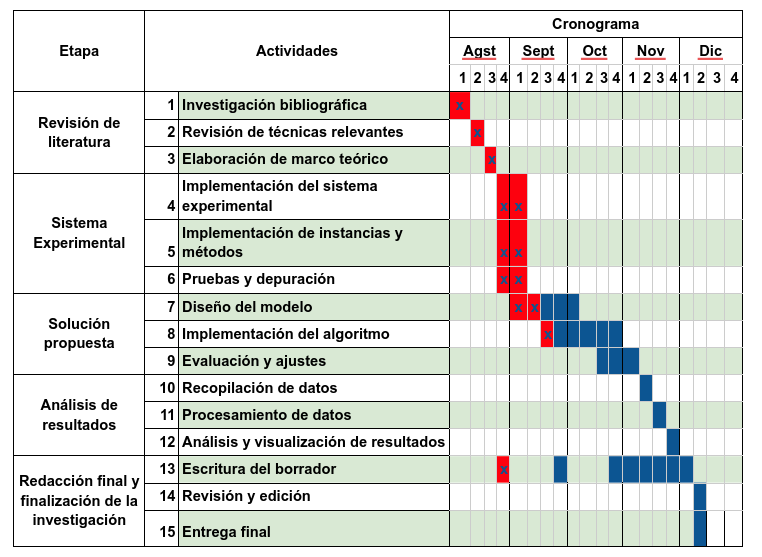
\includegraphics[width=1.1\linewidth]{Images/image.png}
%    \caption{Cronograma actual}
%    \label{fig:cronograma}
%\end{figure}
%\end{center}

%----------------Página de derechos de autor: elegir entre a) o b) y borrar/comentar la opción NO utilizada-----------------
\thispagestyle{empty}
\mbox{}                         % Ayuda a bajar el texto
\vfill                          % Deja el texto al fondo
\textcopyright\ 2023, José Ignacio González Cortés \\ % Derechos de autor
%a)
Ninguna parte de esta memoria puede reproducirse o transmitirse bajo ninguna forma o por ningún medio o procedimiento, sin permiso por escrito del autor.\\\\
%b)
Se autoriza la reproducción total o parcial, con fines académicos, por cualquier medio o procedimiento, incluyendo la cita bibliográfica del documento
\vspace{1cm}    % lo separa del fondo
\restoregeometry % Devuelve los márgenes después de la portada


%----------------Página de calificaciones (opcional), descomentar para generar-----------------

% Editar en Otros -> Calificaciones.tex

%%Las calificaciones entregan la misma información de la portada y se le agrega la nota y la firma. Esta página es opcional.
\begin{titlepage}
	
	\newgeometry{top=1 in, bottom=1 in, left=1 in, right= 1 in} 
	
	\thispagestyle{frontpage}
	
	\begin{center}
		
		\vspace*{4\baselineskip}
	
		
		{\Huge \textbf{TÍTULO PRINCIPAL\\}}%No abreviar, no subrayar, no usar comillas. Se escribe completamente en mayúsculas
		        \vspace*{1.5\baselineskip}

		\large{\textit{subtítulo}}\\ %No abreviar, no subrayar, no usar comillas. Solo la priemra letra usa mayúsculas
		
        \vspace*{1,5\baselineskip}

		\large{\textbf{Por: Autor}}\\ %Nombre como aparece en registro académico
		
		\vspace{1,5\baselineskip}
		
		\large{Tesis presentada a la Facultad de Ciencias Físicas y Matemáticas de la Univerisdad de Concepción para optar al grado académico de Magister en Ciencias con Mención en Física.} %Cambiar a grado académico correspondiente. 
		
		\vspace{1,5\baselineskip}
		Diciembre 2019\\ %Mes y año de la tesis, solo primera letra del mes en mayúsculas
		Concepción, Chile %Ciudad y país de publicación.
\vspace{1,5\baselineskip}

		\large{\textbf{Profesor Guía: Nombre}}\\ %Nombre del profesor que dirigió el trabajo, de la comisión informante y otros asesores precedidos por los títulos correctos de la unidad académica.  
		%Al margen derecho del profesor guía se estampa la firma y/o calificación.
		

	\end{center}
	

	
\end{titlepage}         % Genera la pagina de calificaciones del archivo calificaciones.tex
%\restoregeometry                           % Devuelve los márgenes después de la página

%\pagenumbering{gobble}         % Suprime la numeración de páginas
%\thispagestyle{plain}          % suprime el encabezado
%\clearpage\mbox{}\clearpage    % Agrega página en blanco

%----------------Página de dedicatoria (opcional), descomentar para generar ---------------------------------


\thispagestyle{empty}
\mbox{}
\vfill
\hfill \text{Dedicatoria}

\restoregeometry

%-------------------------------------------------




%-----------------Página de agradecimientos (opcional), se incluye normalmente-------------------

% Editar en Otros -> Agradecimientos.

\pagenumbering{roman}                            % Empieza la enumeración romana en minúsculas, para mayúsculas usar Roman.


\newpage
\addcontentsline{toc}{chapter}{AGRADECIMIENTOS}  % Agrega esta sección al índice
\section*{AGRADECIMIENTOS}                       % Debe ir en mayúsculas por reglamento de la UdeC, tiene asterisco para no ser numerada.


\vspace*{2\baselineskip}

\lipsum[4-5] % Texto para mostrar la página, Borrar cuando se escriban los agradecimientos

\vspace*{3\baselineskip}




%-----------------Página de resumen (abstract)-------------

% Si la unidad académica lo requiere, se edita en  Otros -> Resumen.tex . El mismo resumen puede ser incluido en inglés (abstract) en la página siguiente, para agregarlo hay un espacio destinado en el mismo archivo antes mencionado.

\newpage
\addcontentsline{toc}{chapter}{Resumen} % Agrega esta sección al índice
\section*{Resumen}                      % Con asterisco para que no sea numerada.

    \par\vspace*{\fill} % Mueve las palabras clave al final de la página
    \textbf{\textit{Keywords --}} Knapsack Problem %Agregar todas las palabras claves asosciadas con la tesis aquí.
    
    %-----------Si se desea poner el Abstract Des-comentar lo siguiente-----------
    \newpage
    \addcontentsline{toc}{chapter}{Abstract} %Agrega esta sección al índice
    \section*{Abstract}
    
    \par\vspace*{\fill} % Mueve las palabras clave al final de la página
    \textbf{\textit{Keywords --}} Knapsack Problem % Agregar las palabras claves en inglés

%--------------Página de índice.  

%\nocite{*}     % Des-comentar si se desea que TODAS las referencias sean impresas en la lista de referencias, incluyendo las que no fueron finalmente citadas en el texto.

\newpage
{\setstretch{1.0}   % Interlineado de la lista.
\tableofcontents
}

\newpage
{\setstretch{1.0} 
\listoftables}

\newpage
{\setstretch{1.0} 
\listoffigures}


\newpage
\addtocontents{toc}{\protect\setcounter{tocdepth}{4}}   % La profundidad del índice queda en 4, 1.1.1.1
\pagenumbering{arabic}                                  % Comienza la numeración arábiga (números normales)
\setcounter{page}{1}                                    % Comienza el contador de páginas en 1

% A continuación se dejan nombres de diversos capítulos o secciones, para cambiar el nombre del archivo tan solo se debe hacer en la carpeta "capitulos" y luego llamarlos de la forma correcta en "\subfile{Capitulos/nuevonombre}".
% Los nombres de los archivos no pueden llevar tíldes ni espacios para el correcto funcionamiento del compilador, esto no tiene nada que ver con que tengan o no tilde en el documento final.

\chapter{Introducción}
En este capítulo se presentan los antecedentes generales acerca del Problema polinomial robusto de la mochila, las variantes de las cuales se deriva y metodologías de solución asociadas a estas. Los objetivos generales y específicos de esta memoria y la estructura del documento.


\section{Antecedentes generales}

El problema de la mochila (KP, por sus siglas en inglés, Knapsack Problem) es un problema clásico de la investigación de operaciones. Generalmente, el KP modela la necesidad de elegir un conjunto de elementos con costos y beneficios individuales, con una restricción de capacidad máxima, con el fin de maximizar el beneficio. El KP ha sido ampliamente estudiado por su estructura sencilla, y también debido a que muchos otros problemas de optimización más complejos lo tienen como subproblema \citep*{martello_knapsack_1990}.

El KP tiene muchas  variantes, una ellas es la versión robusta, RKP (por sus siglas en inglés, Robust Knapsack Problem). Este fue formulado originalmente por \cite{eilon_application_1987} para resolver problemas de asignación de presupuesto con aplicaciones reales, muchos de los parámetros del problema están asociados a incertidumbre. El RKP fue planteado para encontrar soluciones que sean factibles para todas las posibles variaciones en los costos de elementos \citep{monaci_exact_2013}.

Otra variante es la versión polinomial de la mochila (PKP, por sus siglas en inglés, Polynomial Knapsack Problem) que incluye el concepto de sinergias, es decir, que la elección de una o más alternativas específicas otorga un beneficio o costo extra según estas relaciones. El PKP sirve para modelar sistemas cuyas alternativas presentan conflictos entre ellas, o que cooperan para generar mayor beneficio \citep{baldo_polynomial_2023}.Así, de este problema surge el polinomial robusto (PRKP, por sus siglas en inglés, Polynomial Robust Knapsack Problem). El PRKP toma en cuenta parámetros inciertos y sinergias polinomiales para modelar problemas de selección de alternativas, que se perjudican o benefician entre sí y además muestran comportamiento estocástico.

Debido a la complejidad espacial del PRKP, se han explorado aplicaciones del problema cuadrático de la mochila (QKP, por sus siglas en inglés, Quadratic Knapsack Problem) \citep{gallo_quadratic_1980} y el problema cúbico de la mochila (CKP, por sus siglas en inglés, Cubic Knapsack Problem) \citep{forrester_strengthening_2022} El QKP presenta sinergias entre dos elementos y ha demostrado ser útil en un gran espectro de aplicaciones como posicionamiento satelital \citep{witzgall_mathematical_1975}, localizaciones de centros de transporte como aeropuertos, ferrocarriles o terminales de carga \citep{rhys_selection_1970}. El CKP es extendido desde el QKP y considera sinergias hasta con tres elementos. Además, posee aplicaciones como en el problema de satisfacción Max 3-SAT \citep{kofler_penalty_2014}, el problema de selección \citep{gallo_fast_1989}, el problema de alineación de redes \citep{mohammadi_triangular_2017}, y la detección y tratamiento de enfermedades de transmisión sexual \citep{zhao_treatments_2008}.

Este trabajo propone la exploración de técnicas de machine learning para resolver el PRKP, encontrar una metodología competitiva con aquellas planteadas en la literatura y obtener resultados comparables.

\section{Objetivos}
\subsubsection*{Objetivo general}
Implementar una heurística basada en machine learning para resolver el PRKP.
\subsubsection*{Objetivos específicos}
\begin{itemize}
	\item Revisar la literatura relacionada con problemas de la mochila similares y metodologías aplicables.
	\item Diseñar una heurística basada en machine learning para el PRKP.
	\item Implementar la heurística propuesta basada en machine learning.
	\item Evaluar los resultados y comparar el rendimiento con las metodologías expuestas anteriormente desde la literatura.
\end{itemize}

\section{Estructura del documento}

El documento consta de 6 capítulos, en los cuales se discutirá, el modelo matemático representando el problema (2), la metodología propuesta para resolverlo (3), un análisis comparativo de los resultados experimentales (4), y finalmente una revisión y discusión para concluir el documento. (5).

\clearpage

\chapter{Problema Polinomial Robusto de la mochila}
Este capítulo comprende la definición formal del problema junto al modelo matemático de programación entera. Además, explora literatura asociada a técnicas y metodologías empleadas para la resolución de otros problemas de la mochila que pueden ser extendidos al PRKP.

\section{Descripción del problema}
	El PRKP se define formalmente como un conjunto de elementos $I = \{1,2,\hdots,N\}$ donde estos tienen un beneficio asociado $P_i \in \mathbb{R}:i\in I$. Además, los elementos poseen un coste de comportamiento estocástico que puede variar de forma continua entre una cota inferior y una superior, $C_i \in [LC_i,UC_i]$, donde $LC_i$ es el costo base, y $UC_i$ el costo máximo. De forma aleatoria solo algunos elementos tienen comportamiento estocástico, aquellos que no, cumplen que $C_i = LC_i$. El parámetro que define cuantos elementos de $I$ pueden tener comportamiento estocástico es $\Gamma\leq N$, es decir $|\{i: C_i > LC_i\}| \leq \Gamma$. 	Además existe un presupuesto máximo $W$ para los costes.
	
	El conjunto de sinergias polinomiales se define como $S = \{ A: A \subseteq I \land |A|>1  \}$. Para cada subconjunto de elementos de $I$, existe un beneficio asociado $PS_A$.
	
	El objetivo del problema es encontrar un subconjunto de elementos $X \subseteq I$ que maximice el beneficio total de los elementos de $X$ sumado a los beneficios de sinergias, que aplican cuando $A\subseteq X$, y que además, para cualquier variación estocástica en costes de los elementos.
	
	\subsection*{Ejemplo de PRKP}
		$$I =\{1,2,3\}$$
		$$W = 10.0$$
		$$\Gamma = 2$$

	\begin{table}[H]
		\centering
	\begin{tabular}{|c|c|c|c|}
		\hline
		$i$ & 1 & 2 & 3 \\
		\hline
		$PS_i$ & 3.0 & 6.0 & 10.0 \\
		\hline
		$LC_i$ & 2.0 & 3.0 & 4.0 \\
		\hline
		$UC_i$ & 5.0 & 4.0 & 7.0 \\
		\hline
	\end{tabular}
	\caption{Beneficios y costos de los ítems}
	\end{table}
	
	\begin{table}[H]
		\centering
		\begin{tabular}{|c|c|}
			\hline
			$A$    & $PS_A$\\
			\hline
			$\{1,2\}$ & 1.0 \\
			\hline
			$\{1,3\}$ & 2.0 \\
			\hline
			$\{2,3\}$ & -1.0\\
			\hline
			$\{1,2,3\}$ & 3.0\\
			\hline
		\end{tabular}
		\caption{Beneficios por sinergias}
	\end{table}
	
	
	
	
    
    \section{Modelo matemático}
    
    
    \cite{baldo_polynomial_2023} describe la formulación del modelo matemático linealizado del PRKP compatible con solvers exactos de programación lineal. El modelo se describe a continuación.
    
    \subsection{Parámetros}
     \begin{itemize}
    	\item $I$, El conjunto de elementos posibles, de cardinalidad $N$
    	\item $P_i$, El beneficio asociado al elemento $i$ %P es de profit
    	\item $LC_i$, El coste nominal del elemento $i$    %Lower Cost
    	\item $UC_i$, El coste máximo del elemento $i$     %Upper Cost
    	\item $W$, El presupuesto o coste máximo asociado al problema.
    	\item $S$, El conjunto de sinergias polinomiales.
    	\item $PS_A$, El beneficio de la sinergia $A$
    	\item $\Gamma$, El número máximo de elementos que pueden variar de su costo base.
    	
    	
    \end{itemize}
    
 	\subsection{Variables de decisión:}

    \begin{equation}
    	\label{equ:x_def}
    	x_i = \left\{ 
    	\begin{array}{lc}
    		1 & \text{si  $i\in X$}\\ \\ 
    		0 &  \text{si $i \notin X$}
    	\end{array} \right.
    \end{equation}
    
    \begin{equation}
    	\label{equ:z_def}
    	\mathcal{Z}_A = \left\{ 
    	\begin{array}{lc}
    		1 & \text{si  $i\in A,  \forall i \in X$}\\
    		0 &  \text{si $\exists i\in A: i \notin X$}
    	\end{array} \right.
    \end{equation}

    
    \begin{equation}
    	\label{equ:pi_def}
    	\rho,\pi_i \in \mathbb{R}^+
    \end{equation}
    
    
	\subsection{Función objetivo}
	
	
	\begin{equation}
		\label{eq:of}
		\text{Maximizar} \sum_i^I{P_ix_i} + \sum_{A\in S} PS_A\cdot \mathcal{Z}_A -
		\sum_i^I {LC_{i}x_i} - \left(\Gamma\rho+\sum_i^I \pi_i\right)
	\end{equation}

    \subsection{Restricciones}
    
    \begin{equation}
   		\label{eq:costs}
  		\sum_{i}^{I}{LC_ix_i} + \Gamma\rho+\sum_i^I \pi_i \leq W
    \end{equation}
    
    \begin{equation}
    	\label{eq:cost_relax}
    	\rho + \pi_i \geq \left(UC_i - LC_i\right)\cdot x_i 
    	\hspace{1cm}
    	 \forall i \in I
    \end{equation}
    
    \begin{equation}
    	\label{eq:fijar_z}
    	\sum_{i\in A} x_i \leq |A| - 1 + Z_{A} \hspace{1cm} \forall A \in S:PS_A < 0
    \end{equation}
   
    \begin{equation}
    	\label{eq:fijar_z_2}
    	Z_{A} \leq x_i \hspace{1cm} \forall i \in A \in S: PS_A > 0
    \end{equation}
    
    \begin{equation}
    	x_i \in {0,1},
    	\forall i \in I,
    	\hspace{0.5cm}
    	Z_{A} \in \{0,1\} \forall A \in S    	
    \end{equation}
    
    \begin{equation}
    	\rho \geq 0, 
    	\hspace{0.5cm}
 		\pi_i \geq 0 \forall i \in I
    \end{equation}
    
    
    La función objetivo en la ecuación \ref{eq:of} representa el beneficio de los beneficios y sinergias de los elementos restando el coste máximo posible que estos puedan tener.
    
    La restricción de presupuesto se define con las ecuaciones \ref{eq:costs} y \ref{eq:cost_relax}, en principio $X$ debe ser robusto a las variaciones en los costes por lo que se usa un acercamiento que asume el peor de los casos, es decir el cálculo del coste será siempre maximizado según las posibles variaciones. En este contexto para linealizar el problema \cite{baldo_polynomial_2023} define las variables de decisión auxiliares \ref{equ:pi_def}, que transforman el coste máximo a un problema de minimización.
    
    Para fijar la variable auxiliar $\mathcal{Z_A}$ se especifican las restricciones \ref{eq:fijar_z} y \ref{eq:fijar_z_2}, que favorece las sinergias con beneficio positivo y desfavorece las con beneficio negativo.
  
\section{Revisión de literatura}


El trabajo de \cite{baldo_polynomial_2023} ha introducido por primera vez una metodología para resolverlo, proponiendo un algoritmo genético y un algoritmo basado en machine learning. Este último utiliza un clasificador random forest que predice la probabilidad de cada elemento de estar presente en la solución óptima. Esta predicción se usa para fijar variables de decisión, reduciendo así el tiempo de ejecución de un solver exacto.

\cite{li_novel_2021} ha estudiado el uso de redes neuronales para obtener predicciones de KPs con funciones objetivo no lineales, obteniendo buenos resultados con una estructura basada en teoría de juegos, junto al uso de redes neuronales adversarias.

\cite{rezoug_application_2022} aborda el KP usando distintas técnicas para evaluar las características de los elementos, entre ellos redes neuronales, regresión de procesos gaussianos, random forest y support vector regression. Así, resuelve el problema original, usando solo un subconjunto de los elementos. Luego, mediante el descenso del gradiente y el uso de características de los elementos, decide cuáles de los elementos excluidos agregar a la solución inicial obtenida. En sus resultados muestra que el modelo machine learning entrega soluciones similares a los otros clasificadores, con menores tiempos de ejecución.

\cite{afshar_state_2020} propuso un algoritmo para generar soluciones para el KP usando un modelo de Deep Reinforcement Learning que selecciona los elementos de forma greedy. El algoritmo propuesto construye las soluciones en base a las decisiones del modelo y genera soluciones con una razón de similitud con el óptimo del 99.9\%. Además, usa una arquitectura de A2C con un paso de cuantización de características, que reduce la complejidad espacial del problema en la red, resultando en modelos que usan menos memoria y se ejecutan más rápido.

Si bien estos trabajos no se relacionan directamente con la variante del problema propuesto, sí evidencian que las técnicas de Machine learning pueden usarse de forma efectiva para caracterizar y construir soluciones para el PRKP.
  



\chapter{Metodología}

En este capitulo se expondrá el algoritmo propuesto para resolver el PKRP, así como las definiciones del modelo machine learning que actúa como clasificador, las características de los ítems que se usarán y el proceso de reducción de instancias.

\section{Algoritmo propuesto}

Se propone un algoritmo iterativo con el objetivo de reducir la complejidad del problema de forma gradual, a costa de un pequeño nivel de confianza sobre la solución final obtenida. El algoritmo usa una red neuronal como clasificador. Que con base en ciertas características de cada elemento, decide la probabilidad de estar o no en la solución final. Estas predicciones se usan para asumir ceros en la solución y reducir la instancia original a una más pequeña mediante una transformación. Este proceso puede ejecutarse un número arbitrario de veces, mientras se mantenga la precisión del modelo, al predecir instancias con cada vez menos elementos.

\begin{algorithm}[H]
	\caption{Algoritmo general}\label{alg:general}
	\begin{algorithmic}[1]
		\State $\tau$ \label{alg1:def_tau} \Comment{Umbral de confianza del clasificador}
		\State $I$ \label{alg1:I} \Comment{Conjunto de elementos inicial}
		\State $S$ \label{alg1:sinergias} \Comment{Conjunto de sinergias}
		\Loop
		\State $\mu \gets \frac{|I|}{\log_{10}{|I|}}$ \label{alg1:def_mu} \Comment{Máximo número de elementos a bloquear por paso}
		\State $F \gets$ Características \label{alg1:full_features} \Comment{Cálculo de características de los elementos}
		\State $\tilde{x} \gets$ Clasificador($F$) \label{alg1:get_pred} \Comment{Generación de predicciones continuas}
		\State $Z \subset I \gets$ Z($\tilde{x},\tau,\mu$) \label{alg1:get_Z} \Comment{Selección de elementos para eliminar}
		\If{$ |Z| = 0$ \textbf{or} $\min(\tilde{x}) > \tau$} \label{alg1:break_condition}
		\State \textbf{break}
		\EndIf
		\State $I \gets I-Z$ \Comment{Reducción de la instancia} \label{alg1:update_I}
		\State $S \gets S - \{A \in S, \exists i \in A: i \in Z\}$ \Comment{Actualización de sinergias}\label{alg1:update_S}
		\EndLoop
		\State $X \gets$ SolverExacto($I$) \label{alg1:exact_solver} \Comment{Resolución exacta del conjunto reducido}
	\end{algorithmic}
\end{algorithm}

El algoritmo \ref{alg:general} inicia con la definición del umbral de confianza del clasificador $\tau$ en la línea \ref{alg1:def_tau}. Se establece el conjunto inicial de elementos $I$ en la línea \ref{alg1:I}, y el conjunto de sinergias $S$ en la línea \ref{alg1:sinergias}.

El bucle principal comienza calculando las características de los elementos en la línea \ref{alg1:full_features}. Posteriormente, el clasificador genera predicciones $\tilde{x}$ en la línea \ref{alg1:get_pred} que se encuentran en el rango $[0,1]$. A continuación, se selecciona un conjunto de elementos $Z$ para eliminar en la línea \ref{alg1:get_Z} en función de las predicciones y el umbral $\tau$.

El umbral $\tau$ se establece por el usuario para definir la precisión y velocidad de ejecución del algoritmo y pertenece al rango de valores $[0,0.5]$.

El tamaño maximo de $Z$ se define por $\mu$ en función del numero de elementos que existe en la instancia reducida, como se muestra en la linea \ref{alg1:def_mu}.

El bucle continúa hasta que el conjunto $Z$ está vacío o el valor mínimo de las predicciones $\tilde{x}$ supera el umbral $\tau$, como se verifica en la línea \ref{alg1:break_condition}. Durante cada iteración, se eliminan los elementos de $Z$ de $I$ y se descartan todas las sinergias que incluyan algún elemento de $Z$.

Finalmente, el algoritmo resuelve exactamente el conjunto reducido $I$ utilizando el \textit{solver} exacto en la línea \ref{alg1:exact_solver}, y el resultado se almacena en $X$.


\section{Clasificador}

El clasificador utilizado es una red neuronal de cinco capas. Para la entrada usa features calculadas para un elemento de la instancia, así, se genera una predicción sobre si el elemento tendrá un valor de cero o uno en la solución final.


\begin{figure}[H]
	\centering
	\begin{tikzpicture}[scale=0.5]
		\foreach \x in {3,...,6} {
			\node[shape=circle,draw=black] (Input\x) at (0,\x)  {};
		}
		\foreach \x in {0,...,9} {
			\node[shape=circle,draw=black] (Hidden1\x) at (2,\x)  {};
			\node[shape=circle,draw=black] (Hidden2\x) at (6,\x)  {};
		}
		
		\node[shape=circle,draw=black] (Output) at (9,4.5)  {};
		\node[shape=rectangle,draw=black] (Transformation) at (12,4.5)  {};
		
		
		\foreach \x in {3,...,6}{
			\foreach \y in {0,...,9}{
				\draw (Input\x) to (Hidden1\y);
			}        
		}
		
		\foreach \a in {0,...,9}{
			\foreach \b in {0,...,9}{
				\draw (Hidden1\a) to (Hidden2\b);}
		}
		
		
		\foreach \x in {0,...,9}{
			\draw (Hidden2\x) to (Output);        
		}
		
		
		
		\draw (Output) to (Transformation);
		
		\node at (-1.5,6) {$f_1(i)$};
		\node at (-1.5,5) {$f_2(i)$};
		\node at (-1.5,4) {$f_3(i)$};
		\node at (-1.5,3) {$f_4(i)$};
		
		\node at (2,10) {Capa $1$};
		\node at (6,10) {Capa $N$};
		\node at (9,10) {Out};
		\node at (12,10) {$\Tilde{y}_{pred}(i)$};
		\node at (10.5,8) {$\tanh()$};
		
		
	\end{tikzpicture}
	\caption{Estructura general de la red}
	\label{fig:network}
\end{figure}

\begin{equation}
	\tilde{x}(i) = \frac{1}{2}\left( \tilde{y}(i) + 1 \right)
	\label{eq:soltransformation}	
\end{equation}

Como se muestra en la Figura la entrada de la red es un vector que contiene todas las features del elemento $i$:
$$
f(i) = \textbf{(}f_1(i),f_2(i), \hdots f_\phi(i))\textbf{)}
$$
donde $\phi$ es del número de features.

Através de la función de activación tangente hiperbólica, la red genera un una salida $\tilde{y}$ que se encuentra en el rango [-1,1], la que es posible reconstruir usando la transformación de la ecuación \ref{eq:soltransformation}. 


En base a esto es útil definir la matriz $F_{\phi \times N}$ como en la ecuación \ref{eq:feature_matrix}:

\begin{equation}
F_{\phi \times N}(I) = 
\left( 
\begin{matrix}
	f(1)\\
	f(2)\\
	\vdots \\
	f(N-1)\\
	f(N)\\
\end{matrix}
\right)
\label{eq:feature_matrix}
\end{equation}


Así, la red es una función definida como:
\paragraph*{Predicción para ítem:}
$$
	Net(f) = \tilde{x_i}: f\in [0,1]^\phi \rightarrow \tilde{x}_i \in[0,1]
$$

\paragraph*{Predicción para todos los ítems de una instancia:}

$$
	Net(F) = \tilde{x}: F\in [0,1]^{\phi\times N} \rightarrow x \in[0,1]^{N}
$$

Las features que se utilizan, codifican los parámetros $P_i$, $LC_i$,$UC_i$, $\Gamma$, además de, $ContSol_i$,$Noise$. Las definiciones se encuentran en el anexo \ref{eq:all_features}.

Entre estas:
\begin{itemize}
	\item $ContSol_i$ se refiere a la solución de la relajación continua del PRKP en que la variable de decisión $x_i$ es continua.
	\item Noise es un generador de números aleatorios, que se usa para definir una entrada vacía en la red neuronal, esto da lugar para reemplazar esta feature por otra asociada al estado del algoritmo general.
\end{itemize}


\subsection{Entrenamiento}

Se realizan dos etapas de entrenamiento sobre un conjunto de instancias. La primera etapa consiste en entrenar la red para predecir la solución óptima de cada instancia, y así crear un clasificador general. En la segunda etapa, la red se afina con instancias generadas desde el algoritmo iterativo de reducción. Además, las soluciones con las que se entrenará la red son generadas por un solver exacto que calcula óptimo para cada instancia. 

\begin{algorithm}[H]
	\caption{Primer entrenamiento}\label{alg:training}
	\begin{algorithmic}[1]
		\State TrainingSet \Comment{Conjunto de instancias de entrenamiento} \label{line:trainingset}
		\State Net 		   \Comment{Red neuronal definida anteriormente} \label{line:net}
		\State Optimizer   \Comment{Optimizador para la red} \label{line:optimizer}
		\State Solver      \Comment{Solver exacto para el problema} \label{line:solver}
		\State Loss      \Comment{Funcion de perdida} \label{line:loss}
		
		\For{Instance $\in$ TrainingSet} \label{line:startloop}
		\State $I \gets Instance_I$ \label{line:i_from_instance}
		\State $x \gets Solver(I)$ \Comment{Vector booleano $x$ con la solución óptima de la instancia} \label{line:solveinstance}
		\For{$i \in I$} \label{line:startinnerloop}
		\State $\tilde{x_i} \gets Net(f(i))$  \Comment{Predicción de la red de $x_i$ desde las features} \label{line:prediction}
		\State $loss \gets Loss(x_i,\tilde{x_i})$ \label{line:calculateloss}
		\State $Net \gets Optimizer(Net,loss)$ \Comment{Un paso de optimización de la red} \label{line:optimizationstep}
		\EndFor \label{line:endinnerloop}
		\EndFor \label{line:endloop}
		\State $Net$ \Comment{Red entrenada} \label{line:trainednet}
	\end{algorithmic}
\end{algorithm}

El algoritmo \ref{alg:training} de entrenamiento comienza designando un conjunto de instancias en la linea \ref{line:trainingset} cada una de las estas define el conjunto de parámetros del modelo de programación lineal. Se define la red que se usará en la linea \ref{line:net}, inicializándose con pesos aleatorios.En la linea \ref{line:loss} se declara la función de perdida, que corresponde a la diferencia lineal entre el valor predicho y el valor real.

En la linea \ref{line:optimizer} se declara el optimizador encargado de reajustar los pesos de la red en cada paso de entrenamiento, se usa el algoritmo Adam introducido por \cite{kingma2017adam}, que funciona como alternativa al descenso de gradiente estocástico. Finalmente se declara el solver exacto a usar, Gurobi 10.0.3.

A continuación, se inicia un bucle sobre cada instancia del conjunto de entrenamiento en la línea \ref{line:startloop}. Para cada instancia,
se obtiene el conjunto de elementos así como sus otros parámetros, definiendo $I$ de la instancia, en la línea \ref{line:i_from_instance}.
Se obtiene la solución óptima $x$ para la instancia usando el solver en la línea \ref{line:solveinstance}.


Posteriormente, se inicia un bucle interno sobre los elementos de la instancia en la línea \ref{line:startinnerloop}. Dentro de este bucle, la red neuronal realiza predicciones $\tilde{x_i}$ sobre las características de la instancia utilizando la función \(f(i)\) en la línea \ref{line:prediction}. Se calcula la perdida entre la predicción y la solución óptima en la línea \ref{line:calculateloss}, y la red se actualiza mediante un paso de optimización utilizando Adam en la línea \ref{line:optimizationstep}.

Este proceso de predicción, cálculo de pérdida y optimización se repite para todos los índices en el bucle interno. Una vez completado, se regresa al bucle externo para la siguiente instancia del conjunto de entrenamiento.

Después de que se han procesado todas las instancias del conjunto de entrenamiento, la red neuronal $Net$ se considera entrenada y se devuelve como resultado del algoritmo en la línea \ref{line:trainednet}.




\begin{algorithm}[H]
	\caption{Segundo entrenamiento}\label{alg:tunning}
	\begin{algorithmic}[1]
		\State $\tau$ \label{alg1:def_tau_2} \Comment{Umbral de confianza del clasificador}
		\State TrainingSet \Comment{Conjunto de instancias de entrenamiento}
		\State Net \Comment{Red neuronal pre-entrenada}
		\State Optimizer \Comment{Optmizador para la red}
		\State Loss \Comment{Función de perdida}\label{line:alg2:loss}
		\For{Instance $\in$ TrainingSet}
				\State $I \gets Instance_I $
				\Loop \Comment{Bucle de reducción}
				\State $\mu \gets \frac{|I|}{\log_{10}{|I|}}$ \label{alg2:def_mu} \Comment{Maximo numero de elementos a bloquear por ciclo}
					\State $\tilde{x} \gets Net(F(I))$  \Comment{Vector de predicción de la red} \label{line:alg2:initial_pred}
					\State $Z \subset I \gets Z(\tilde{x},\tau,\mu)$ \label{start_reduction_alg}
					\If{$ |Z| = 0$ \textbf{or} $\min(\tilde{x}) > \tau$ }
						\State $\textbf{break}$ 
					\EndIf
					\State $I \gets I-Z$ \Comment{Reducción de la instancia} \label{alg1:update_I_2}
					\State $S \gets S - \{A \in S, \exists i \in A: i \in Z\}$ \Comment{Actualización de sinergias} \label{end_reduction_alg}
				\State $x \gets Solver(I)$  \Comment{Solución óptima de la instancia reducida} \label{solve_smaller}
				\State $\tilde{x} \gets Net(F(I))$ \Comment{Predicción para la instancia reducida} \label{pred_smaller}
			\For{$i \in I$}
				\State $loss \gets Loss(x_i,\tilde{x_i})$     \Comment{Cálculo de la perdida} \label{smaller_loss}
				\State $Net \gets Optimizer(Net,loss)$		  \Comment{Actualización de los pesos de la red} \label{smaller_optim}
			\EndFor
			\EndLoop
		\EndFor
		\State $Net$ \Comment{Red entrenada}
	\end{algorithmic}
\end{algorithm}

El segundo proceso de entrenamiento descrito en el algoritmo \ref{alg:tunning} sigue la estrategia del algoritmo general \ref{alg:general}. Inicialmente se declaran los parámetros $\tau$ y $\mu$, asi como el conjunto de instancias de entrenamiento, la red neuronal pre-entrenada, el optimizador y la función de perdida, en las líneas \ref{alg1:def_tau_2} a \ref{line:alg2:loss}. Se ejecuta el bucle de reducción por cada instancia, usando red la predicción en la línea \ref{line:alg2:initial_pred}. Al igual que en el algorimo general \ref{alg:general} , se usa esta predicción, para generar una instancia reducida, este proceso ocurre en las líneas \ref{start_reduction_alg} a \ref{end_reduction_alg}. Luego se calcula la solución óptima para la instancia reducida, en la línea \ref{solve_smaller}, asi como la predicción de la red en la línea \ref{pred_smaller}. Finalmente, se realiza un paso de optimización por cada elemento en la instancia reducida donde se calcula la perdida entre la predicción y el valor óptimo en la linea \ref{smaller_loss} y se ajustan los pesos de la red en la línea \ref{smaller_optim}.
Después de ejecutar este proceso por todas las instancias del conjunto de entrenamiento, y actualizar los pesos usando todos los pasos de reducción de las instancias, se obtiene la red entrenada final.

Un cambio que mejora la precisión de la red resolver instancias reducidas, es reemplazar la feature \ref{feature:6} que correspondía un valor aleatorio, por una métrica que representa cuanto se ha reducido la instancia desde su tamaño original. Por esto en las ocaciones que se calcula $F(I)$ para el segundo entrenamiento, $f_6$ es reemplazada por la feature de la ecuación \ref{feature:7}, donde la instancia actual se refiere $|I|$ de cada ciclo del bucle de reducción.

\begin{equation}
	\label{feature:7}
	f_7(i) = \frac{\text{N instancia Original}}{\text{N instancia actual}}
\end{equation}




 \section{Construcción de Z y reducción de instancias}
 
 EL proceso de reducción descrito en las lineas \ref{alg1:update_I} y \ref{alg1:update_S} del algoritmo general \ref{alg:general} requiere definir el proceso de creación de Z con base en los parámetros.
 
 \begin{algorithm}[H]
 	\caption{$Z(\tilde{x},\tau)$}\label{alg:z}
 	\begin{algorithmic}[1]
 		\State $B \gets \{ i \in I: \tilde{x}_i \leq \tau \}$ \label{create_B}
 		\State $B \gets Sort(A)$  \Comment{Ordenar de forma ascendente en base a los valores de $x_i$}
 		\State $Z \gets \{\}$	  
 		\State $c \gets 0$	\label{define_c}
 		\ForAll{$b \in \{1,2,3...,|B|\}$}		  \Comment{Agregar los $\mu$ items con menor $x_i$}
 		\State $Z \gets B_b$ \label{add_to_z}
 		\State $c \gets c + 1$ \label{add_c}
 		\If{$c = \mu$}\label{if_c}
 		\State \textbf{break} \label{break}
 		\EndIf
 		\EndFor
 		\State Z
 	\end{algorithmic}
 \end{algorithm}
 
 El algoritmo \ref{alg:z} se encarga de construir Z de forma que contenga los elementos ordenados con predicciones mas cercanas a cero que estén bajo el umbral $\tau$, con un tamaño máximo de $\mu$. Comienza creando un conjunto $B$ que posee todos los elementos cuya predicción $\tilde{x}_i$ es menor que $\tau$ en la linea \ref{create_B}. En la línea B este conjunto es ordenado de manera ascendente, de forma que $\tilde{x}_{B_b} < \tilde{x}_{B_{b+1}}   \forall b \in [1,|B|]$. Así, en un bucle que itera sobre los indices de B, los elementos son agregados a Z en la linea \ref{add_to_z} de forma estrictamente ordenada. Este blucle termina si B se queda sin elementos que agregar a Z, o si la cardinalidad de Z supera el número máximo elementos definido por $\mu$. De esto se encarga el contador c, definido en la linea \ref{define_c} el que cuenta cada elemento agregado a Z en la linea \ref{add_c} y detiene el blucle en el control de flujo de la linea \ref{if_c}.
 
 
 Al aplicar el proceso de reducción a una instancia de forma repetida, es posible que sucedan los siguientes casos.
 
  \begin{itemize}
 	\item En cada paso la proporción de unos vs ceros en la solución óptima sera cada vez mayor, hasta el punto en que será irreducible.
 	
 	\item  $\Gamma$ no cambia al eliminar ceros. Es posible que se llegue a que $\Gamma > |I|$, dejando la posibilidad de reformular el problema como PKP.
 \end{itemize}
 
 
 
\clearpage
\chapter{Resultados Experimentales}
En este capitulo se presentará la comparación cuantitativa de resultados, se re-contextualizarán los métodos de \cite{baldo_polynomial_2023} con base en las diferencias de hardware y se mostrará la evaluación del algoritmo propuesto.

\section{Instancias}

Las instancias reales que se resuelven provienen de un generador de instancias implementado por \cite{baldo_polynomial_2023} cuyas sinergias tienen en su mayoría beneficios de cero. Las instancias con $I$ mayor a 1000, tienen una generación exponencial de sinergias. Para $300 \le I \le 1000$, se usa una generación cuadrática de sinergias. Para instancias con menos de 300 elementos, se generan sinergias de forma lineal.

Para comparar el rendimiento del algoritmo propuesto con los solvers existentes propuestos por \cite{baldo_polynomial_2023}, se usó el mismo conjunto de instancias propuesto, además de otras de mayor tamaño con el objetivo de comparar rendimiento para problemas de un orden de magnitud más grande.

\section{Comparaciones}

Se calcularon los resultados para todas las instancias de \cite{baldo_polynomial_2023}, usando los métodos de BaldoGA y BaldoML, además de el algoritmo propuesto.

\subsection*{Resultados generales}
\subsubsection*{Comparación de solver exacto con trabajo anterior}
En la figura \ref{fig:solver_times} se muestran los tiempos para resolver instancias usando el solver exacto, en contraste con \cite{baldo_polynomial_2023}, que solo resolvió instancias de hasta 650 elementos con tiempos hasta 7000s, en este caso los tiempos están acotados a cerca de 550 segundos.

\begin{figure}[h]
	\centering
	\begin{subfigure}{.5\textwidth}
		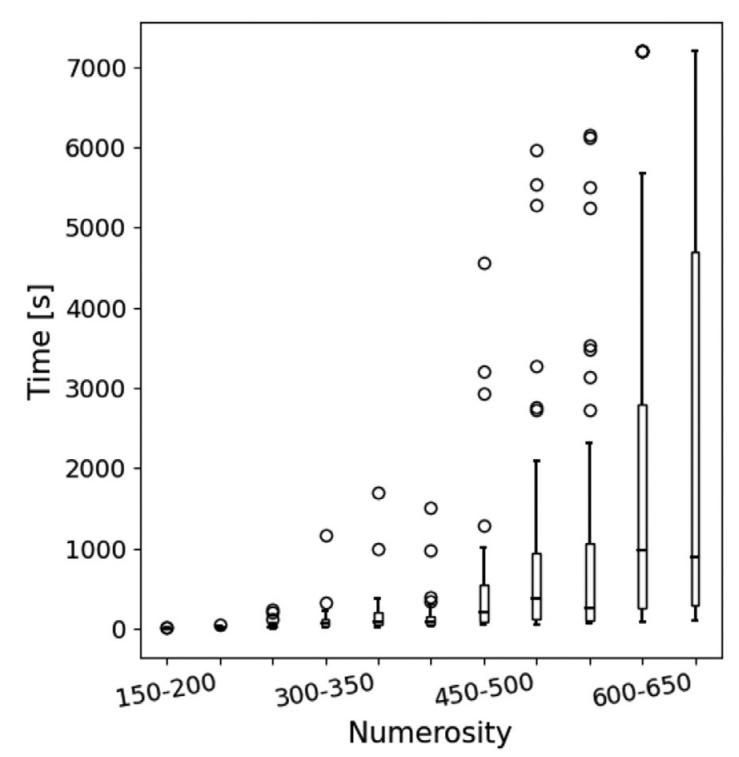
\includegraphics[width=1\linewidth]{graphs/baldo_solver_times.png}
		\caption{Ejecución Gurobi \cite{baldo_polynomial_2023}}
	\end{subfigure}%
	\begin{subfigure}{.5\textwidth}
		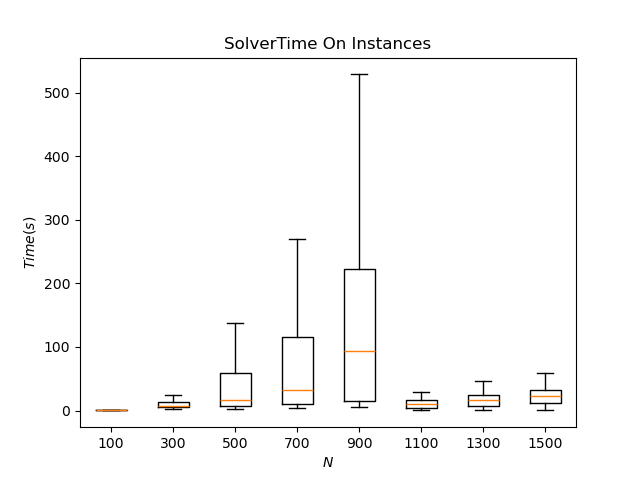
\includegraphics[scale=0.656]{graphs/solver_times.png}
		\caption{Ejecución Gurobi actual}
	\end{subfigure}%
	\caption{Tiempos de ejecución solver exacto}
	\label{fig:solver_times}
\end{figure}

\subsubsection*{Rendimiento normalizado}

Se presenta en las figuras \ref{fig:full_gap} y \ref{fig:full_timegap} la comparación general de rendimiento de los métodos. BaldoGA tiene un $\bar{gap} = 3.29\%$ y BaldoML tiene un gap promedio del 2.1\%. Estos resultados son congruentes con el estudio de \cite{baldo_polynomial_2023}, mostrando comparabilidad con los resultados.


\begin{figure}[H]
	\centering
	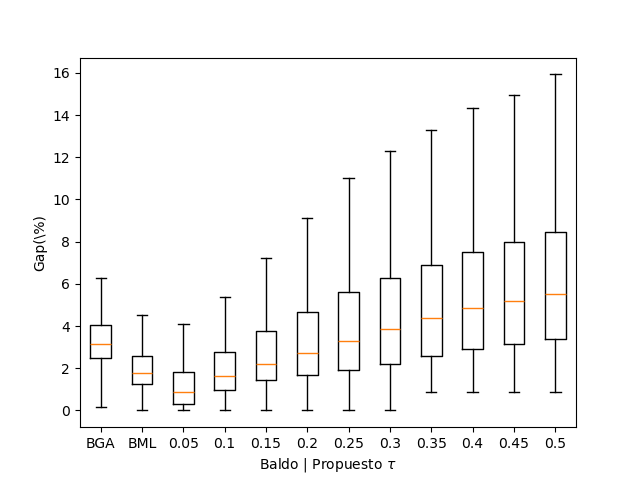
\includegraphics[scale=0.7]{graphs/full_gap_comparison.png}
	\caption{Gap \% de todos los métodos presentados}
	\label{fig:full_gap}
\end{figure}

\begin{figure}[H]
	\centering
	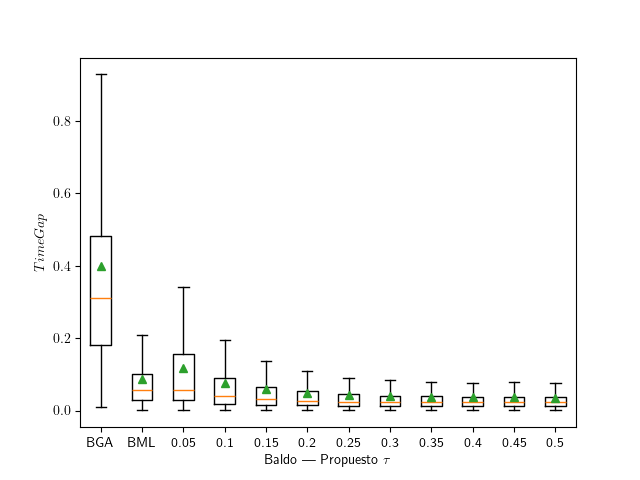
\includegraphics[scale=0.7]{graphs/full_timegap_comparison.png}
	\caption{TimeGap(\%) de los métodos usados}
	\label{fig:full_timegap}
\end{figure}





\begin{table}[H]
	\begin{adjustbox}{width=\columnwidth,center}
		\begin{tabular}{cccccccccccc}
			
			\multicolumn{3}{c}{Método}&  &\multicolumn{8}{c}{N}\\
			\cline{1-3} \cline{5-12}
			\multicolumn{3}{c}{} &  & 100  & 300  & 500  & 700  & 900  & 1100 & 1300 & 1500\\
			\hline
			\multirow{4}{*}{BaldoGA} & \multirow{2}{*}{Gap(\%)} & $\mu$ && 1.74 & 3.07 & 3.04 & 3.42 & 3.74 & 3.4 & 4.1 & 3.9 \\
			&                          & $\sigma$ & & 1.15 & 0.905 & 0.866 & 0.844 & 1.09 & 1.07 & 6.89 & 1.18 \\
			\cline{2-3}
			& \multirow{2}{*}{Time(s)} & $\mu$ && 0.44 & 3.3 & 4.5 & 7.18 & 9.86 & 5.61 & 7.22 & 8.89 \\
			&                          & $\sigma$ & & 0.207 & 1.32 & 1.75 & 2.93 & 4.08 & 2.19 & 2.44 & 3.21 \\
			\hline		 	 
			\multirow{4}{*}{BaldoML} & \multirow{2}{*}{Gap(\%)} & $\mu$ && 3.16 & 3.0 & 2.2 & 2.0 & 1.85 & 1.41 & 1.37 & 1.39 \\
			&                          & $\sigma$ & & 1.87 & 1.19 & 0.907 & 0.72 & 0.66 & 0.56 & 0.6 & 0.49 \\
			\cline{2-3}
			& \multirow{2}{*}{Time(s)} & $\mu$    && 0.099 & 0.36 & 0.48 & 0.79 & 1.19 & 1.5 & 2.12 & 2.85 \\
			&                          & $\sigma$ && 0.0147 & 0.0577 & 0.119 & 0.277 & 0.47 & 0.881 & 1.33 & 1.67 \\
			\hline		 						 
			
			\multirow{4}{*}{$\tau=0.05$} & \multirow{2}{*}{Gap(\%)} & $\mu$ && 2.45 & 1.79 & 1.36 & 1.40 & 1.41 & 1.40 & 1.23 & 1.02 \\
			&                          & $\sigma$ & & 2.50 & 1.70 & 1.35 & 1.36 & 1.38 & 1.36 & 1.26 & 1.15 \\
			\cline{2-3}
			& \multirow{2}{*}{Time(s)} & $\mu$ && 0.20 & 0.88 & 1.46 & 2.61 & 3.80 & 3.41 & 4.67 & 6.28 \\
			&                          & $\sigma$ & & 0.09 & 0.37 & 1.05 & 2.06 & 2.97 & 2.73 & 3.47 & 4.49 \\
			\hline		 						        
			
		\end{tabular}
	\end{adjustbox}
	\caption{Comparación general por número de elementos}
	\label{tab:comparison_table}
\end{table}

La tabla \ref{tab:comparison_table} es un extracto de los resultados en \ref{tab:full_comparison_table}, que muestra BaldoML, BaldoGA y El algoritmo propuesto con un $\tau=0.05$. Es posible notar que el propuesto encuentra soluciones con un menor gap promedio que BaldoML, esto a costa de tener desviaciones estándar más altas y tiempos de ejecucion comparativamente mas altos.


%Los tiempos de ejecucion....

En la figura \ref{fig:distributions} se ilustra la principal diferencia entre baldoML y el propuesto. Los métodos tienen un gap medio de 2.05\% y 1.51\% respectivamente, esta diferencia de 0.54\% de ambas medias es significativa con un $p = 1.8\cdot10^{-26} < 0.05$ en una prueba T-student, rechazando la hipótesis de igualdad de medias.

\begin{figure}[H]
	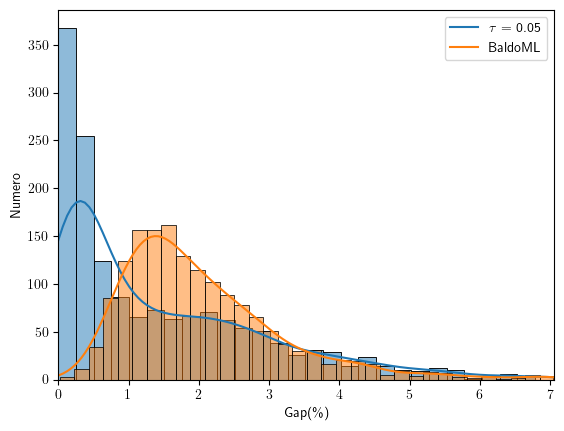
\includegraphics{graphs/distributions.png}	
	\label{fig:distributions}
	\caption{Contraste distribución gap BaldoML vs Propuesto}
\end{figure}

Respecto a los tiempos de ejecución, baldo resolvió todas las instancias en 1859.86 segundos, lo que corresponde a 1.1719s en promedio por instancia. Mientras que el método propuesto tardó 4611.1s en resolver el conjunto completo de instancias, con un promedio de 2.9 segundos. Debido a que las instancias tienen distintos tamaños y los tiempos de ejecución varían exponencialmente según este, se presenta en la figura \ref{fig:distributions_times} una distribución de los tiempos normalizados. Se aprecia visualmente que ambos tiempos se distribuyen de forma similar, con un desplazamiento positivo de la media del método propuesto. En promedio baldo se tarda 8.5\% del tiempo del solver óptimo en encontrar una solución, mientras que el propuesto 15.93\%.

\begin{figure}[H]
	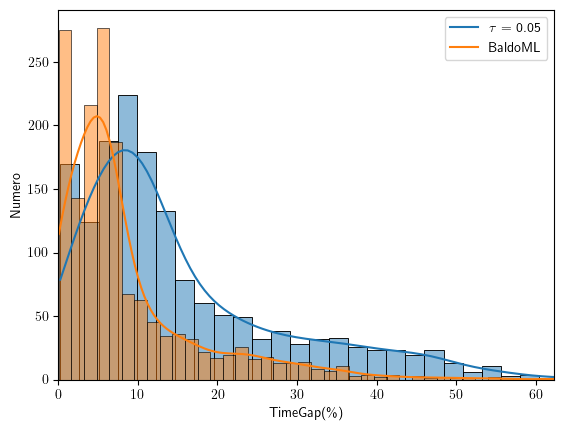
\includegraphics{graphs/distributions_times.png}	
	\label{fig:distributions_times}
	\caption{Contraste distribución tiempos de ejecución normalizados BaldoML vs Propuesto}
\end{figure}

\subsection*{Instancias grandes}

Se resolvieron 50 instancias de $|I| = 20000$ con el objetivo de comparar las capacidades de escalamiento de los métodos BaldoML y el propuesto. Debido a la inviabilidad de utilizar el solver exacto para estos tamaños de instancias los valores de la función objetivo son comparados a razón de $\frac{\text{Propuesto}_{Of}}{\text{BaldoML}_{Of}}$ para obtener su gap relativo.

En todos los casos, baldoML encontró mejores soluciones para las instancias, pero como se ilustra en la figura \ref{fig:comparison} la diferencia entre esos es marginal. Las soluciones del método propuesto fueron en promedio un 4.47\% más pequeñas que las soluciones obtenidas por baldoML, variando entre un 6.2\% y 2.85\% en el peor y mejor de los casos respectivamente.

\begin{figure}[H]
	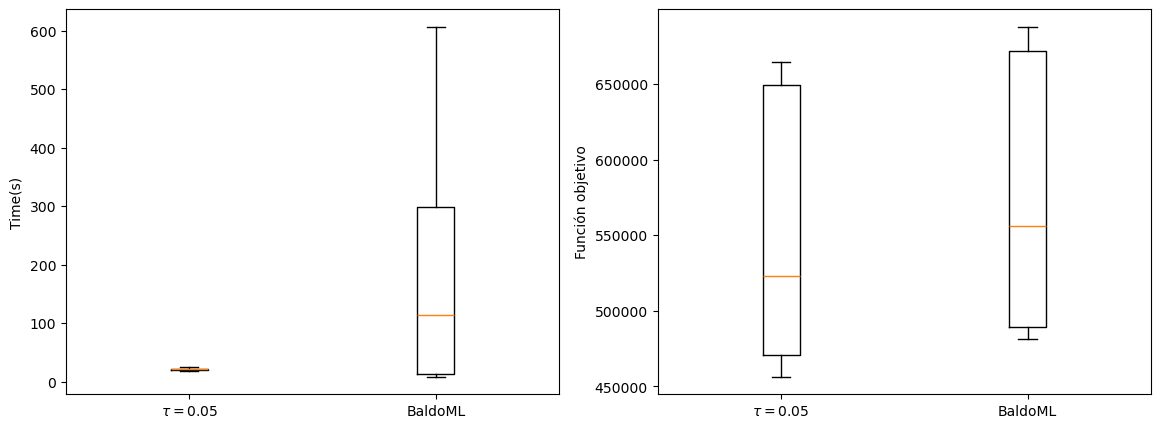
\includegraphics[scale=0.5]{graphs/comparison.png}	
	\caption{Comparación BaldoML y Propuesto en instancias de 20000 elementos}
	\label{fig:comparison}
\end{figure}



En cuanto a los tiempos de ejecución, la diferencia ha tenido mayor magnitud. Se estableció un límite de ejecución de 600 segundos por instancia. Mientras que baldoML tardo 2 horas y 26  minutos en resolver todo, el método propuesto usó poco menos de 18 minutos. Además, el tiempo de ejecución del propuesto, parece mantenerse relativamente constante en estos tamaños, mientras los tiempos de baldoML se distribuyen de forma más amplia, con una desviación estándar muy alta.


\begin{table}[H]
	\centering
	\begin{tabular}{|c|c|c|}
		\hline
		&BaldoML& Propuesto\\
		\hline
		Tiempo total & 8809s & 1064.02s\\
		\hline
		Tiempo promedio&176.18s & $21.28s$ \\
		\hline
		Desviación estandar &164.44s& $1.60s$\\
		\hline
	\end{tabular}
	\caption{Estadísticas tiempos de ejecución en instancias grandes}
\end{table}







\chapter{Conclusiones}
En esta memoria de título se describe un algoritmo basado en machine learning para abordar el problema polinomial robusto de la mochila, usando un clasificador que opera de forma iterativa sobre una instancia para reducir su complejidad. Se ha definido la estructura de la red neuronal, el algoritmo general de operación, los 2 métodos de entrenamiento y el método de reducción de la instancia.
 
Respecto a los resultados, el algoritmo muestra un rendimiento objetivamente superior al algoritmo genético propuesto por \cite{baldo_polynomial_2023} en terminos de precisión y tiempos de ejecucion y si bien tiende a tardar mas que BaldoML, presenta mejores soluciones. Además, tiene mejores características de escalamiento en términos de rendimiento y tiempos de ejecución para instancias de tamaño no contemplado en el conjunto de entrenamiento. La metodología propuesta es entonces más adecuada para abordar instancias que son in-factibles para resolver con un solver exacto pese a tener altos tiempos de ejecución en instancias pequeñas.

En el futuro sería importante explorar el uso de técnicas más avanzadas de machine learning para abordar el problema, implementar sistemas de decisión automática para los parámetros de los solvers mostrados y además explorar el uso de características derivadas de estimadores basados en machine learnig, como la arquitectura A2C introducida por \cite{mnih_asynchronous_2016}, con el fin de predecir características sin necesidad de derivarlas de la solución óptima.




    
    
\clearpage

\newpage
\renewcommand\refname{Referencias}          % Nombre para la lista de referencias, también se utiliza "Bibliografía"
{\setstretch{1.0}                           % Interlineado de las referencias 
\addcontentsline{toc}{chapter}{Referencias} % Cambia el nombre de la lista de referencias en el índice 
\bibliography{Referencias.bib}              % Agrega las referencias al documento, estas se ubican en el archivo Referencias.bib
}

\newpage
\renewcommand{\appendixpagename}{Apéndices}     % Nombre al inicio.
\addcontentsline{toc}{chapter}{Apéndices}       % Agrega "Apéndices" al índice

\appendix   % Empieza el ambiente de apéndices, desde ahora en adelante los capítulos, secciones, tablas, figuras, etc. vuelven a empezar su numeración

\chapter{Material}

\section{Rendimiento de métodos en distintos tamaños de entrada}
\begin{figure}[h]
	\centering
	\begin{subfigure}{.5\textwidth}
		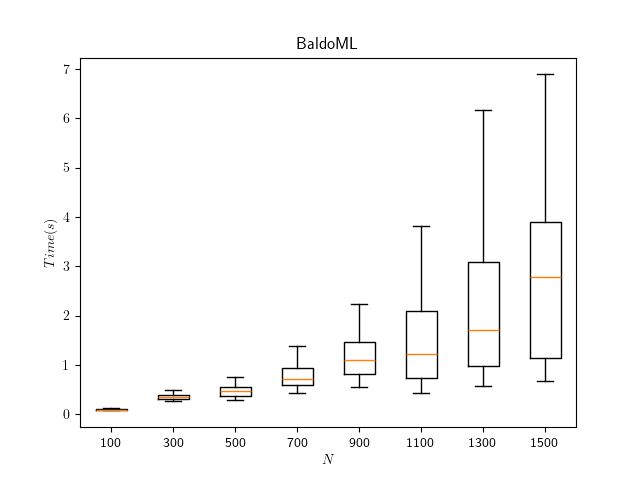
\includegraphics[width=1\linewidth]{graphs/BaldoML_time.png}
		\caption{Tiempo vs Numero de elementos}
	\end{subfigure}%
	\begin{subfigure}{.5\textwidth}
		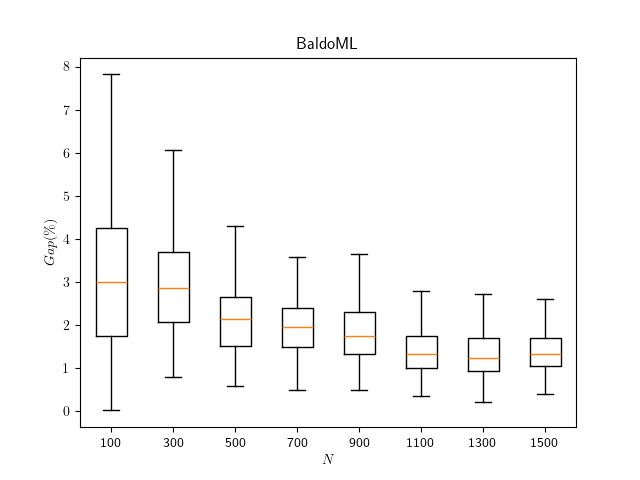
\includegraphics[width=1\linewidth]{graphs/BaldoML_gap.png}
		\caption{Gap vs Número de Elementos}
	\end{subfigure}%
	\caption{Rendimiento BaldoML}
	\label{fig:perf_baldoml}
\end{figure}

\begin{figure}[h]
	\centering
	\begin{subfigure}{.5\textwidth}
		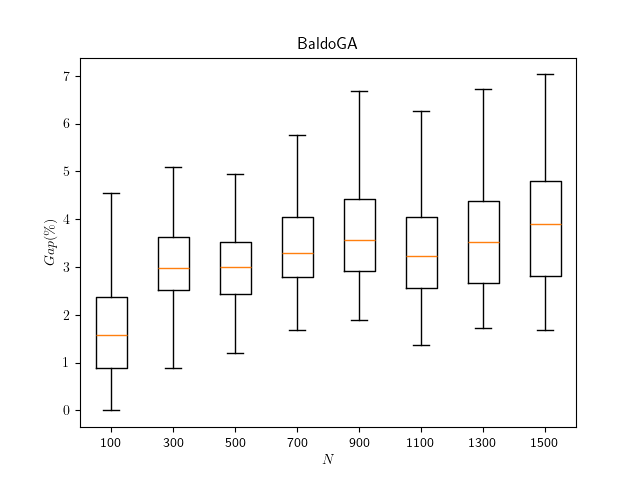
\includegraphics[width=1\linewidth]{graphs/BaldoGA_gap.png}
		\caption{Tiempo vs Numero de elementos}
	\end{subfigure}%
	\begin{subfigure}{.5\textwidth}
		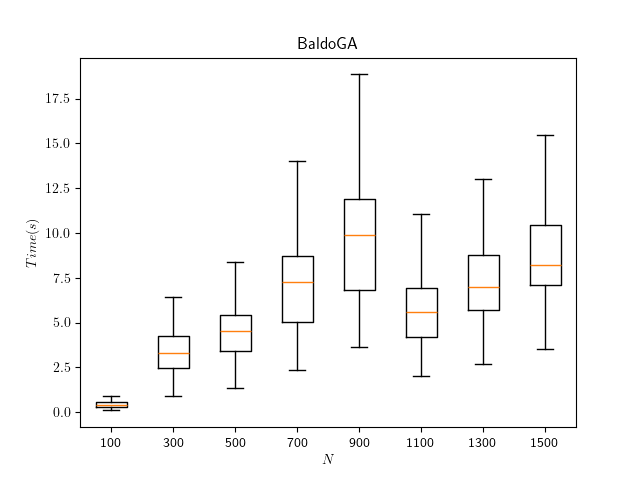
\includegraphics[width=1\linewidth]{graphs/BaldoGA_time.png}
		\caption{Gap vs Numero de Elementos}
	\end{subfigure}%
	\caption{Rendimiento BaldoGA}
	\label{fig:perf_baldoga}
\end{figure}


\newcommand{\resultadosZ}[1]{
	\begin{figure}[h]
		\centering
		\begin{subfigure}{.5\textwidth}
			\includegraphics[width=1\linewidth]{graphs/Z_threshold#1_time.png}
			\caption{Tiempo vs Numero de elementos}
		\end{subfigure}%
		\begin{subfigure}{.5\textwidth}
			\includegraphics[width=1\linewidth]{graphs/Z_threshold#1_gap.png}
			\caption{$Gap(\%)$ vs Numero de Elementos}
		\end{subfigure}%
		\caption{Rendimiento Algorimo propuesto $(\tau=#1)$}
		\label{fig:perf_z_#1}
	
	\end{figure}
}

\resultadosZ{0.05}
\resultadosZ{0.1}
\resultadosZ{0.15}
\resultadosZ{0.2}
\resultadosZ{0.25}
\resultadosZ{0.3}
\resultadosZ{0.35}
\resultadosZ{0.4}
\resultadosZ{0.45}
\resultadosZ{0.5}


\begin{comment}
		\begin{table}[h]
			\centering
			\begin{adjustbox}{width=\columnwidth,center}
				\begin{tabular}{|ccc|cccccccc|}
					\hline
					\multicolumn{3}{|c}{Método} & \multicolumn{8}{c|}{N}\\
					\hline
					\multicolumn{3}{|c|}{\text{}}  & 100  & 300  & 500  & 700  & 900  & 1100 & 1300 & 1500 \\
					\hline
					\multirow{4}{*}{BaldoGA}   & \multirow{2}{*}{Gap(\%)} 	  & $\mu$    & 1.74 & 3.07 & 3.04 & 3.42 & 3.74 & 3.4 & 4.1 & 3.9\\
					&                                                     	  & $\sigma$ & 1.15 & 0.905 & 0.866 & 0.844 & 1.09 & 1.07 & 6.89 & 1.18 \\
					\cline{3-11}
					& \multirow{2}{*}{Time(s)}  							  & $\mu$    & 0.44 & 3.3 & 4.5 & 7.18 & 9.86 & 5.61 & 7.22 & 8.89\\
					&                           							  & $\sigma$ & 0.207 & 1.32 & 1.75 & 2.93 & 4.08 & 2.19 & 2.44 & 3.21 \\ 
					\hline		 						 
					\multirow{4}{*}{BaldoML} & \multirow{2}{*}{Gap(\%)}       & $\mu$    & 0.15 & 0.0723 & 0.0751 & 0.105 & 0.037 & 1.03 & 2.01 & 2.02\\
					&                                                         & $\sigma$ & 0.339 & 0.151 & 0.202 & 0.218 & 0.0736 & 10.0 & 14.0 & 14.0 \\
					\cline{3-11}
					& \multirow{2}{*}{Time(s)}                                & $\mu$    & 0.475 & 3.74 & 7.9 & 12.9 & 21.1 & 18.6 & 30.8 & 38.2\\
					&                                                         & $\sigma$ & 0.195 & 3.25 & 5.86 & 11.3 & 15.9 & 60.6 & 83.0 & 82.2 \\
					\hline
					\multirow{4}{*}{$\tau_{0.05}$} & \multirow{2}{*}{Gap(\%)} & $\mu$    & 2.48 & 1.34 & 1.12 & 1.09 & 1.14 & 1.12 & 1.02 & 0.839\\
					&                                                         & $\sigma$ & 2.48 & 1.08 & 0.922 & 0.868 & 0.996 & 1.01 & 0.965 & 0.837 \\
					\cline{3-11}
					& \multirow{2}{*}{Time(s)}                                & $\mu$    & 0.138 & 0.665 & 1.32 & 2.46 & 4.08 & 3.43 & 4.84 & 6.68\\
					&                                                         & $\sigma$ & 0.104 & 0.391 & 0.874 & 1.74 & 2.98 & 2.8 & 3.83 & 4.69 \\
					\hline
					\multirow{4}{*}{$\tau_{0.1}$} & \multirow{2}{*}{Gap(\%)}  & $\mu$    & 4.2 & 2.19 & 1.89 & 1.87 & 1.92 & 1.85 & 1.8 & 1.58\\
					&                                                         & $\sigma$ & 3.17 & 1.18 & 1.14 & 1.3 & 1.33 & 1.3 & 1.35 & 1.19 \\
					\cline{3-11}
					& \multirow{2}{*}{Time(s)}                                & $\mu$    & 0.0914 & 0.511 & 0.929 & 1.6 & 2.5 & 2.07 & 2.84 & 3.88\\
					&                                                         & $\sigma$ & 0.0735 & 0.281 & 0.562 & 0.848 & 1.52 & 1.7 & 2.12 & 3.11 \\
					\hline
					\multirow{4}{*}{$\tau_{0.15}$} & \multirow{2}{*}{Gap(\%)} & $\mu$    & 5.65 & 2.81 & 2.49 & 2.42 & 2.65 & 2.42 & 2.45 & 2.15\\
					&                                                         & $\sigma$ & 3.36 & 1.34 & 1.47 & 1.55 & 1.76 & 1.6 & 1.67 & 1.32 \\
					\cline{3-11}
					& \multirow{2}{*}{Time(s)}                                & $\mu$    & 0.0653 & 0.415 & 0.767 & 1.37 & 2.18 & 1.65 & 2.26 & 2.9\\
					&                                                         & $\sigma$ & 0.0491 & 0.207 & 0.392 & 0.66 & 1.25 & 1.22 & 1.6 & 1.97 \\
					\hline
					\multirow{4}{*}{$\tau_{0.2}$} & \multirow{2}{*}{Gap(\%)}  & $\mu$    & 6.68 & 3.4 & 2.99 & 2.9 & 3.2 & 2.94 & 2.97 & 2.75\\
					&                                                         & $\sigma$ & 3.55 & 1.65 & 1.76 & 1.76 & 2.04 & 1.79 & 1.8 & 1.49 \\
					\cline{3-11}
					& \multirow{2}{*}{Time(s)} 								  & $\mu$    & 0.0537 & 0.36 & 0.689 & 1.22 & 1.95 & 1.41 & 1.9 & 2.32\\
					&                                                   	  & $\sigma$ & 0.0313 & 0.148 & 0.3 & 0.527 & 1.03 & 0.933 & 1.28 & 1.25 \\
					\hline
					\multirow{4}{*}{$\tau_{0.25}$} & \multirow{2}{*}{Gap(\%)} & $\mu$    & 7.47 & 3.94 & 3.42 & 3.37 & 3.7 & 3.43 & 3.52 & 3.33\\
					&                                                   	  & $\sigma$ & 3.81 & 1.97 & 2.0 & 1.9 & 2.29 & 1.97 & 1.93 & 1.7 \\
					\cline{3-11}
					& \multirow{2}{*}{Time(s)} 								  & $\mu$    & 0.0472 & 0.335 & 0.65 & 1.1 & 1.74 & 1.2 & 1.6 & 2.01\\
					&                                                         & $\sigma$ & 0.0202 & 0.118 & 0.278 & 0.383 & 0.655 & 0.614 & 0.818 & 0.904 \\
					\hline
					\multirow{4}{*}{$\tau_{0.3}$} & \multirow{2}{*}{Gap(\%)}  & $\mu$    & 8.27 & 4.36 & 3.76 & 3.78 & 4.17 & 3.87 & 4.06 & 3.87\\
					&                                                   	  & $\sigma$ & 4.03 & 2.23 & 2.16 & 2.08 & 2.41 & 2.13 & 2.05 & 1.88 \\
					\cline{3-11}
					& \multirow{2}{*}{Time(s)} 								  & $\mu$    & 0.044 & 0.317 & 0.611 & 1.04 & 1.58 & 1.06 & 1.41 & 1.79\\
					&                                                   	  & $\sigma$ & 0.0142 & 0.0979 & 0.232 & 0.299 & 0.407 & 0.426 & 0.538 & 0.574 \\
					\hline
					\multirow{4}{*}{$\tau_{0.35}$} & \multirow{2}{*}{Gap(\%)} & $\mu$    & 8.89 & 4.75 & 4.12 & 4.21 & 4.62 & 4.32 & 4.53 & 4.4\\
					&                                                   	  & $\sigma$ & 4.17 & 2.49 & 2.32 & 2.25 & 2.6 & 2.28 & 2.15 & 2.1 \\
					\cline{3-11}
					& \multirow{2}{*}{Time(s)} 								  & $\mu$    & 0.0428 & 0.302 & 0.575 & 0.984 & 1.51 & 0.982 & 1.3 & 1.61\\
					&                                                   	  & $\sigma$ & 0.0112 & 0.0699 & 0.177 & 0.199 & 0.286 & 0.251 & 0.272 & 0.211 \\
					\hline
					\multirow{4}{*}{$\tau_{0.4}$} & \multirow{2}{*}{Gap(\%)}  & $\mu$    & 9.5 & 5.02 & 4.45 & 4.57 & 5.04 & 4.71 & 4.96 & 4.88\\
					&                                                   	  & $\sigma$ & 4.26 & 2.67 & 2.49 & 2.4 & 2.75 & 2.43 & 2.27 & 2.27 \\
					\cline{3-11}
					& \multirow{2}{*}{Time(s)}                                & $\mu$    & 0.0413 & 0.295 & 0.55 & 0.943 & 1.45 & 0.938 & 1.24 & 1.59\\
					&                                                         & $\sigma$ & 4.950e-03 & 0.0571 & 0.128 & 0.123 & 0.161 & 0.163 & 0.077 & 0.0932 \\
					\hline
					\multirow{4}{*}{$\tau_{0.45}$} & \multirow{2}{*}{Gap(\%)} & $\mu$    & 10.0 & 5.27 & 4.77 & 4.94 & 5.42 & 5.05 & 5.32 & 5.27\\
					&                                                         & $\sigma$ & 4.35 & 2.89 & 2.67 & 2.56 & 2.88 & 2.58 & 2.38 & 2.43 \\
					\cline{3-11}
					& \multirow{2}{*}{Time(s)}                                & $\mu$    & 0.0416 & 0.292 & 0.535 & 0.921 & 1.43 & 0.918 & 1.23 & 1.59\\
					&                                                         & $\sigma$ & 4.670e-03 & 0.0485 & 0.0889 & 0.0716 & 0.0948 & 0.0513 & 0.0667 & 0.0893 \\
					\hline
					\multirow{4}{*}{$\tau_{0.5}$}& \multirow{2}{*}{Gap(\%)}   & $\mu$    & 10.4 & 5.49 & 5.03 & 5.29 & 5.73 & 5.36 & 5.64 & 5.61\\
					&                                                         & $\sigma$ & 4.5 & 3.08 & 2.83 & 2.75 & 2.98 & 2.75 & 2.52 & 2.61 \\
					\cline{3-11}
					& \multirow{2}{*}{Time(s)}                                & $\mu$    & 0.0416 & 0.285 & 0.528 & 0.917 & 1.44 & 0.913 & 1.23 & 1.59\\
					&                                                         & $\sigma$ & 4.760e-03 & 0.0321 & 0.0676 & 0.0413 & 0.0745 & 0.0479 & 0.0702 & 0.0943 \\
					\hline
				\end{tabular}
			\end{adjustbox}
			
			\caption{Tabla completa de resultados}\label{tab:full_comparison_table}
		\end{table}
\end{comment}







\chapter{Ecuaciones}
\section{Features Clasificador}
\begin{multicols}{2}
	\label{eq:all_features}
	\begin{equation}
		f_1\left(i\right)   = \frac{P_i}{W}
		\label{feature:1}
	\end{equation}
	
	\begin{equation}
		f_2\left(i\right)   = \frac{LC_i}{W}
		\label{feature:2}
	\end{equation}
	
	\begin{equation}
		f_3\left(i\right)   = \frac{UC_i}{W}
		\label{feature:3}
	\end{equation}
	
	\begin{equation}
		f_4\left(i\right)   = \frac{\Gamma}{N}
		\label{feature:4}
	\end{equation}
	
	\begin{equation}
		f_5\left(i\right)   = \text{ContSol}_i
		\label{feature:5}
	\end{equation}
	
	\begin{equation}
		f_6\left(i\right)   = \text{Random}\left(i\right)
		\label{feature:6}
	\end{equation}

\end{multicols}

\clearpage



\end{document} 
